\documentclass[sigconf]{acmart}
\usepackage[utf8]{inputenc}
\usepackage{pmboxdraw}
\usepackage[T1]{fontenc}

\usepackage[english]{babel}
\usepackage{blindtext}

% Copyright
\renewcommand\footnotetextcopyrightpermission[1]{} % removes footnote with conference info
\setcopyright{none}
%\setcopyright{acmcopyright}
%\setcopyright{acmlicensed}
%\setcopyright{rightsretained}
%\setcopyright{usgov}
%\setcopyright{usgovmixed}
%\setcopyright{cagov}
%\setcopyright{cagovmixed}

\settopmatter{printacmref=false, printccs=false, printfolios=true}

\usepackage{hyperref}
\usepackage{fancyvrb}
\usepackage{adjustbox}
\DeclareUnicodeCharacter{2529}{|}

% Support for easy cross-referencing
\usepackage[capitalize]{cleveref}
\crefname{section}{Sec.}{Secs.}
\Crefname{section}{Section}{Sections}
\Crefname{table}{Table}{Tables}
\crefname{table}{Tab.}{Tabs.}
\Crefname{appendix}{Appendix}{Appendices}

% DOI
\acmDOI{}

% ISBN
\acmISBN{}

%% {} with no args suppresses printing of the price
\acmPrice{}


\begin{document}
\title{A lightweight python based cluster and workload manager}

%\titlenote{}
\subtitle{CS 630 Distributed Systems Project Report}

\author{Ali Hassani\\alih@uoregon.edu}

% The default list of authors is too long for headers}
\renewcommand{\shortauthors}{Hassani}

\begin{abstract}
    Cluster managers are among the key software components in compute clusters.
    They provide an interface to administrators to manage compute nodes, their resources and software, and allow real-time
    monitoring of both physical and logical states. Workload managers on the other hand provide an interface to the users by
    allowing allocating available resources for user-defined compute jobs.
    The goal is to allow users to somewhat abstract their computations from physical nodes by defining jobs on a single ``head''
    node, which, once scheduled, will be distributed among requested resources.
    Herein we present an open source cluster and workload manager written in Python with minimal dependencies, set up to use
    containerization as a means to create virtual nodes within the same physical node.
    Among its applications are partitioning physical resources within one physical node (CPU cores, memory, GPUs) into virtual
    nodes mimicking a compute cluster, and creating an easy and lightweight solution for running and testing 
    parallel/distributed jobs on minimal hardware.
\end{abstract}

\maketitle

\section{Introduction}

High-performance computing (HPC) can be described as a design system where clusters of powerful computers are unified as a
supercomputer for highly compute-intensive experiments.
They continue to play a key role in science and technology, and without them, arguably many of the advances seen since the
beginning of the 21st century would not have come close to being feasible.
A perfect example is the surge in AI since the early 2010s, when, thanks to NVIDIA's general purpose GPUs and CUDA programming 
model~\cite{kirk2007nvidia}, researchers started parallelizing the training of highly advanced neural networks of record sizes
and on large sums of data. This surge continues today, and with it bringing about more demand for HPC systems and
infrastructure to maximize parallelism and compute power~\cite{klenk2017relaxations}.

At their very core, compute clusters are simply comprised of a set of networked computers, 
each with certain computational capabilities and resources.
In many HPC scenarios, clusters are set up in such a way that clients can request resources for experiments.
This distributed environment where compute nodes collaborate to create a single unified system through which researchers, 
engineers, and scientists conduct their experimentation, are therefore crucial to the advancement of science and technology.
These environments are comprised of many elements, including, but not limited to, their infrastructure, meaning the physical
nodes, drives, network infrastructure, and the like, along with a software layer to construct, maintain, and manage the 
distributed environment.
The software layer, also referred to as \textbf{cluster manager}, handles most of the coordination, anywhere from providing 
interfaces to systems engineers and administrators to set up and maintain the cluster, to setting up operating systems and 
scheduling services for clients who would eventually utilize the resources.
An example of that is the Bright Cluster Manager~\cite{bright}, which is commonly installed in NVIDIA clusters.
Another role of the cluster manager is to handle workloads, for which it can rely on a separate workload manager.
SLURM (Simple Linux Utility for Resource Management)~\cite{yoo2003slurm} is one such service, and is among the most widely 
adopted among large-scale supercomputers and compute clusters.

In this work, we introduce a lightweight python-based cluster and workload manager with minimal dependencies, that can be
deployed on most computers capable of running containerized services such as Docker~\cite{merkel2014docker}, and utilizes the
infrastructure that they provide.
This service can be used to divide up resources existing on a single computer for the purposes of training, dividing and
scheduling the use of resources among multiple clients, and can also be used to develop distributed programs.

\section{Background}

As mentioned, cluster management software is typically installed on all of the networked computers, or \textit{compute nodes}. 
It is also a typical assumption that one or more computers manage, organize, and control compute nodes, and provide interfaces
to clients who wish to use the cluster of compute nodes. Such nodes referred to as \textit{head nodes}, where the cluster
management software is also deployed.
Cluster management software relies on a workload management service or module such as SLURM~\cite{yoo2003slurm}, which provides 
the user interface for clients in order to allow them to request resources, and schedule their jobs accordingly.
While the cluster management software keeps track of all nodes, their health status, and so on, it also passes their
information, such as IP addresses, resource availability, and the like, to the workload manager.
Together, the cluster management software and workload manager run persistent monitoring and messaging processes in order to
maintain a unified compute cluster that serves the purpose of maximizing the clients' ability to complete their computations in
a timely manner. 

In this work, our approach is to create a single lightweight software component with minimal dependencies that can coordinate
and create such an environment, and is deployable to most computers through the use of containerization tools such as
Docker~\cite{merkel2014docker}. Through using docker, our approach can simulate separate compute and head nodes even with
different operating systems, and allow clients to design and run distributed jobs.


\section{Methodology}

In this section, we describe the proposed approach towards building a minimal-dependency cluster management (CM) service that
would operate using the infrastructure provided by Docker~\cite{merkel2014docker}.
We divide the service into two components: infrastructure and CM software, which are described in the following subsections.
An overview of the proposed system is presented in \cref{fig:overview}.

\begin{figure*}[ht]
    \centering
    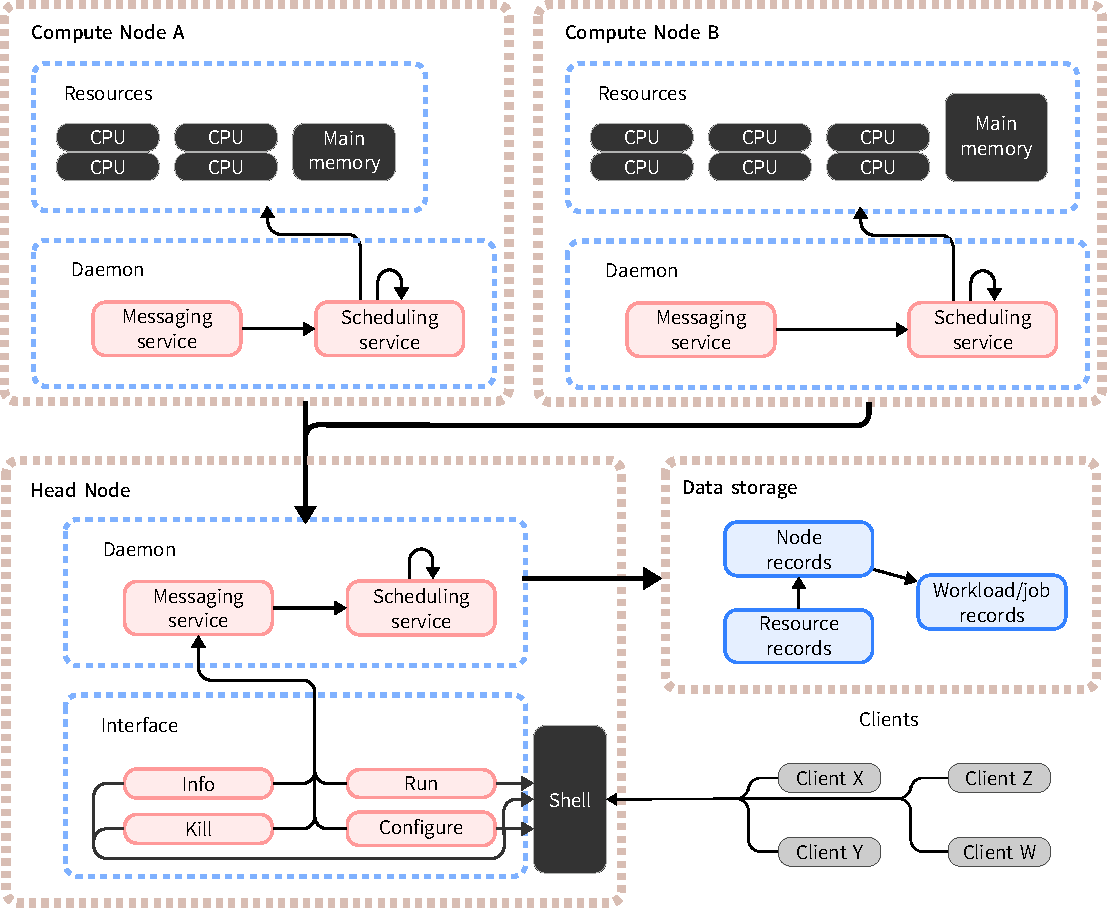
\includegraphics[width=0.95\textwidth]{figures/overview.pdf}
    \caption{
        \textbf{An overview of the components in the proposed cluster manager.}
        Each node will run the CM daemon, which consists of a messaging service, and scheduling service.
        Upon initialization, the daemon is responsible for detecting available resources, starting the services, and registering
        itself with the head node. Head node, once itself initialized, will store information on nodes and resources in a local
        storage. Clients can then use the available interfaces to see available resources, nodes, create/stop jobs, and
        configure the CM (depending on their privileges.)
    }
    \label{fig:overview}
\end{figure*}

\subsection{Infrastructure}
As mentioned, the service relies on Docker~\cite{merkel2014docker} for both infrastructure and containerization as a means to
mimic individual physical nodes.
This is achieved through creating container images for head and compute nodes separately.
While images for both package the software, which will be described in the next subsection, they can differ slightly in terms of
dependencies. For example, routines that are implemented only to be executed from the head node need not be packaged into the
software on compute nodes, and drivers required to access or utilize computational resources on compute nodes should not be part
of the head node image.

Container images used in this work are based on the official Ubuntu image from Docker hub, and include the additional Python
3.10, along with dependencies that are Python packages.
The primary dependencies are: Zero-MQ (ZMQ), PyYAML, \verb|psutil|, and \verb|rich|.
ZMQ socket interfaces are used to implement messaging services used in both head and compute nodes,
PyYAML handles parsing the main configuration file that holds the CM default values and settings,
\verb|psutil| provides a Python interface over the operating system's ``process status'' tool, which is used to monitor the 
state of running jobs.
\verb|rich| is a command line pretty-printer used in CM interfaces in order to print available resources and jobs in tables.

In addition to head node and compute node containers, we also containerize the database. 
Head node keeps records of resources, nodes, and jobs in a MongoDB database, which is implemented in a separate container.

Finally, all services are connected through a docker network between the head node and compute nodes, and a separate network
connecting the head node and database element.
In addition, we set up mounts to a persistent shared home directory between head node and compute nodes, following standard
practice in compute clusters.

The aforementioned container services are organized using \verb|docker-compose|.
Services are exposed to clients through accessing an interactive terminal into the head node container, and compute nodes are
simulated by scaling compute node containers.

\subsection{Software components}

As previously stated, the shared software is primarily written in Python or using Python interfaces.
Herein we describe the different components present in the software, starting with communication.

\subsubsection{Communication}
For the purposes of this project, we write two socket classes on top of ZMQ's request and reply sockets.
The reason for that is to provide abstractions to other software components for communication, and reduce code replication, as
these sockets will be the basis for communication in the entire system.

By default, the sockets are set up to serialize and transmit pickled python objects, and all communication is assumed to be
\textbf{synchronous} with \textbf{fail-stop} semantics, meaning requests are time-bounded and timed out requests are handled as
if the destination is offline.
The time bound chosen is 100 milliseconds on our experimental setup, which was the lowest point over multiple bounds that
resulted in no failures detected in the system. Values tried were 1 ms, 10 ms, 50 ms, 100 ms, 500 ms, and 1000 ms.
All requests that were strictly between two nodes (typically compute and head) can be easily handled with a 10 ms time bound.
However, requests that incur follow up requests to all compute nodes (4 in our experiments), for example checking the status of
every node, rarely succeed with a 10 ms or even 50 ms time bound. However, 100 ms appears to be a relatively optimal choice.
Under heavy workloads in our experimental setup, one or two compute nodes may fail to register with the head node due to the
increased response time when all 4 compute nodes try to register at approximately the same time. They can however successfully
retry and for the remaining period the system functions as expected.

\subsubsection{Abstractions and structures}
For ease of modification, extension, and reduced code replication, we introduce the following abstractions and structures into
the project:

\paragraph{Job:} an object that holds information about a client-initiated process/job.
Jobs hold a unique identifier, which we define to be a non-negative integer that is incremented per job submission,
but this identifier is assigned to the job once it is accepted by the service.
Jobs also hold an optional name, the UID of the user submitting it (so that it may be executed by the same user across nodes
instead of as root), the command (i.e. \verb|python compute.py|), working directory and environment variables, optional time
limit, and resources requested.
Resources requested consist of number of nodes, number of processes per node, number of CPU cores reserved per node, and amount
of memory reserved per node.
Job instances also hold a status property, which can take values such as \verb|Pending|, \verb|Started|, \verb|Running|,
\verb|Completed|, \verb|Killed|, or \verb|Unknown|.

\paragraph{Resource:} an object containing a type (CPU, memory, GPU, and the like), a capacity (CPU cores, amount of memory),
and a key-value store for allocations.
The key-value store matches job identifiers with the amount of the resource reserved (number of cores, amount of memory).
Resources therefore implement methods for checking allocations, confirming allocations, and removing allocations.

\paragraph{Node:} an object containing a unique identifier (hostname), type (head or compute), and resources.
Upon initialization of any service, every node is able to identify itself based on environment variables.
This is achieved through Docker's ability to pre-define environment variables for every container.
Resources should be identified through either drivers, or a pre-defined configuration, but for the purposes of this work, we
define all compute node containers as having 2 CPUs, each with 1 core, and 1 main memory of size 512 megabytes.

Nodes implement multiple methods, some of which are designed to be called both locally and through a remote procedure call (RPC).
Some of those methods are described as follows:
\begin{itemize}
    \item Status check: report whether node is idle or in use. If RPC calls fail, node is assumed to be down.
    \item Resource allocation: reserve some of node's resources by calling the resource allocation methods.
    \item Job start: queue and start a job process
    \item Job end: kill or stop process if still running, free resources allocated for it.
\end{itemize}

The reason for this formulation is that Node instances can be created in different routines throughout the software, or even
fetched from the database. Instead of writing new procedures for finding a node's address and port, starting a socket, and
sending a request for an action, all of this can be done through simply calling the methods on the node.
If the method is being called on the same node, the local procedure will be called, and if called from a remote node, RPC will
be initiated.

\paragraph{Queue:} As described in \verb|Node|, jobs are queued and then started. 
Queue is an object that holds key-value mappings between job identifiers and their corresponding \verb|Job| instance, which
holds the information necessary to start the jobs (command, working directory, user id, environment variables), as well as
process ids (PIDs) corresponding to jobs that have already started for monitoring.

\verb|Queue| instances run on compute nodes only, and are shared among subprocesses, which is why it is implemented with methods
that save its context to file given any one instantiation. This is necessary simply because the main service daemon is broken
into different subprocesses, as all communication in this system is synchronous. This will be further clarified in
\cref{sec:daemons}.

\paragraph{Message:} all communication done in this system is done through sending instances of this object.
\verb|Message| instances include the originating node's unique identifier, an action (see \cref{supp:actions}), an optional
response, and an optional content field for transmitting structured or unstructured data.

To further ease communication, RPC calls, and reduce code duplication, most message sending is factored into a single method.
It starts by taking in two arguments: node and message. A socket is started at a random port, and then binded to the 
node's address and receiving port, and message transmission is attempted, and the result is returned. 
There is an additional routine for sending messages to the head node,
which solely relies on the existing configuration and only takes the message as input.
This is heavily used in RPC calls and interfaces.


\subsubsection{Daemons}
\label{sec:daemons}
Herein we describe the properties of the daemons, which are the central component of the entire system.
Both head nodes and compute nodes start off by launching the daemon, and their aliveness is defined by the daemon functioning as
expected.
Daemons start off with the same procedure on both types of nodes, which is reading environment variables and the configuration
file. As described previously, the configuration file holds presets, defaults, and settings, all of which are described in
detail in \cref{supp:configuration}.

Once the daemon identifies itself, meaning it has constructed its own \verb|Node| instance, it can start communicating.
It then launches procedures according to its type (head or compute).

\paragraph{Head daemon:}
Head node depends on the data storage element, therefore it starts by initializing a connection to the database, which in this
case is only initializing the MongoDB connection string.
Once completed, the daemon starts its two subprocesses: \textbf{messaging service}, and \textbf{scheduling service}.
The messaging service simply starts a receiving socket at a fixed receiving port (defined in the configuration, and fixed across
nodes of the same type), and blocks on receiving messages.
Message handling is done according to the action specified in the \verb|Message| instance (see \cref{supp:actions}).
The scheduling service on the other hand repeats its procedure in small time intervals (defined in the configuration). The
procedure is comprised of fetching pending jobs, and calling the workload manager on them in order to attempt scheduling jobs,
and if successful, communicating the job to the assigned nodes.
The workload manager is described in \cref{sec:wlm}.

\paragraph{Compute daemon:}
Unlike head nodes, compute nodes do not need to connect to the database, since the head node is the only entity in the entire
system with direct access to the database. This helps maintain our assumption of a single coordinator, and therefore avoiding
race conditions.
Once a compute daemon is started, and identifies itself, it first communicates with the head node to ``register'' itself.
Registration is simply comprised of announcing its existence and resources to the head node.
Nodes simply transmit a \verb|Message| with the appropriate action, along with their \verb|Node| instance, which includes their
identifier, as well as available resources.
Upon receipt, head node attempts to create a new node record in the database, or update an existing one with the same node id
(in case of a failure and reboot of a compute node.)
Once registered successfully, the compute daemon also breaks into two \textbf{messaging} and \textbf{scheduling} subprocesses,
similar to the head node. However, there's a few differences in both.
Messaging service on compute nodes, while similar in functionality to the head node, handle a different set of actions compared
to the head node, and therefore have their own set of action to handler mappings.
Scheduling service on the other hand is almost entirely different from that of the head node.
It is comprised of two separate subprocesses, one responsible for starting jobs, and another responsible for monitoring jobs.

The former repeats its procedure in small time intervals, similar to the head node instance in that regard, and checks its local
\verb|Queue| instance for pending jobs.
If any are found, it attempts to start the jobs as described by their instance, and logs their process identifiers (PIDs.)
Once all replicas of a single job have started and their PIDs are logged, the process reports the job back to the head node,
indicating that the job has started running. This triggers an update in the database from the head node, and once all nodes
assigned to the job have made the same report, the head node changes the job status to ``running'' in the database.

The second scheduling subprocess, which is responsible for job monitoring, repeats its procedure is time intervals larger than
the previous, leading to its procedures called less frequently (intervals are configurable).
Its procedure checks the local \verb|Queue| instance for \textit{running} jobs, those with PIDs, and simply monitors the process
state and runtime. We note that runtime can be both checked both from the process state and also logged by the scheduler when it
starts the job in the first place. We choose the latter and therefore avoid resolving possible differences between timestamps on
different PIDs corresponding to the same job.
Once each job's state and runtime is logged, the monitoring procedure attempts to report jobs that are no longer running
(completed, killed, or other similar states) back to the head node. It also attempts to terminate jobs that have exceeded the
time limit, if there is one.
Head nodes on the other hand again keep track of nodes reporting job completion, and once all assigned nodes report back,
triggers a job status update.

\subsubsection{Workload manager}
\label{sec:wlm}
We implement a simple greedy scheduler in this work, but in theory any scheduler would be applicable to this system, and can
simply replace the existing one.
The scheduler is designed to maintain a FIFO (first in first out) ordered queue, which is guaranteed by the ordering in the
database according to job ids.
Given the ordered set of pending jobs, and an updated the list of available nodes and their available resources through
RPC, workload manager assigns resources to the first job whose requirements can be met.
In other words, given any job, the workload manager either finds the specified resource requirements and starts the job, or
fails to schedule the job, which means the job will be put back into the queue and checked again later.
The procedure also includes communicating with each node separately once to check resource availability, and once to reserve
resources and start the job.
Because the system is built under the assumption that there is a single head node, or more generally, single coordinator, race
conditions are ruled out as a possibility, meaning while the scheduler is attempting to reserve node $x$'s resources for job
$i$, no job $j$ can possibly reserve and take node $x$'s resources before job $i$ gets a chance.
A flowchart of the steps taken in the workload manager is presented in \cref{fig:wlm}.

\begin{figure}[ht]
    \centering
    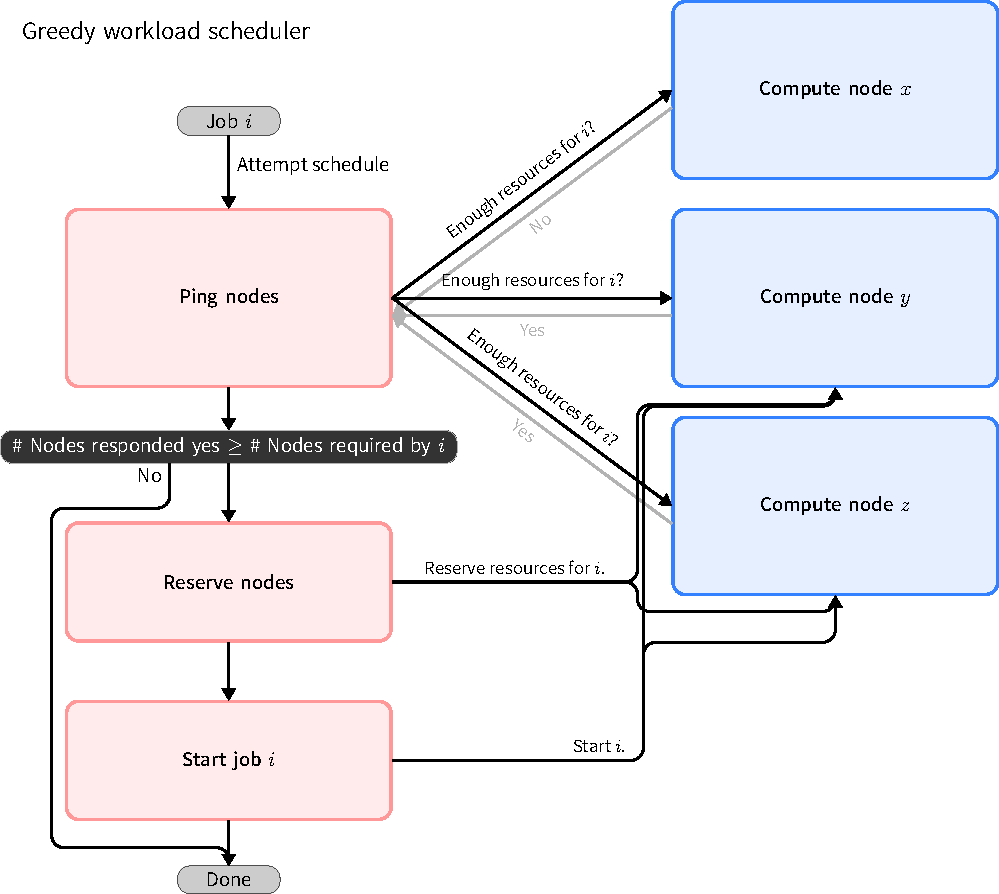
\includegraphics[width=0.475\textwidth]{figures/wlm.pdf}
    \caption{
        \textbf{A flowchart of the workload manager.}
        Pending jobs are held in a FIFO queue, and upon the removal of every job from the queue, the workload manager attempts
        to reserve nodes for the given job. It starts by sending messages to all available nodes, along with the job's resource
        requirements, such as number of CPU cores and amount of memory. Compute nodes simply respond whether or not resources
        are available. If in the end, more nodes than required by the job are available, as many as required by the job are
        reserved and the job instance is transmitted to said nodes, which will then proceed to start the processes.
        Reserved nodes will remain in communication with the workload manager on the head node, reporting the status of the
        running processes, and when and if they stop, or go over the time limit.
        If the workload manager fails to schedule the input job, it simply adds it to the end of the queue.
    }
    \label{fig:wlm}
\end{figure}

\subsubsection{Interfaces}
Interfaces are programs that would be exposed to clients for interacting with the system.
Similar to SLURM~\cite{yoo2003slurm}, we implemented separate programs for starting and stopping jobs, as well as checking the
overall status of the system.
Those programs and their arguments are described below:

\verb|cminfo|: Prints an overview of the cluster, broken into head nodes, compute nodes, and ``valid''
jobs (either running or pending). Takes no arguments. A sample output from this tool is presented in \cref{fig:cminfo}.

\verb|cmrun|: Allows users to set up jobs. Arguments are the following:
\begin{itemize}
    \item Command is the only required argument. It is the command or commands that will be executed on compute nodes.
    \item \verb|-a| \verb|--alias|: an optional job name. Defaults to the first word in command.
    \item \verb|-n| \verb|--nodes|: number of nodes to replicate the job on. Defaults to 1.
    \item \verb|-p| \verb|--processes|: number of replica processes per node. Defaults to 1.
    \item \verb|--num-cpus-per-node|: number of CPU cores to reserve per node. Defaults to 1.
    \item \verb|--mem-per-node|: amount of memory to reserve per node. Defaults to 100.
    \item \verb|-t| \verb|--time-limit|: Job time limit in hours. Defaults to 0 (non-positive values represent no time limit).
\end{itemize}

\verb|cmkill|: Allows users to terminate / stop their jobs. Only takes 1 argument: job id.

\verb|cmconfigure|: Allows configuring elements in the cluster, such as nodes, their resources, users, and the
    like. This tool was not implemented due to certain limitations imposed by the operating system when creating a shared
    user management service.

\begin{figure}[ht]
    \centering
    \begin{adjustbox}{max width=0.475\textwidth}
\begin{BVerbatim}
                              Head nodes                               
┏━━━━━━━━━━━━━━┳━━━━━━━━┳━━━━━━━━┳━━━━━━━━┳━━━━━━━━━━━━━┳━━━━━━━━━━━━━┓
┃     Node     ┃ Status ┃ # CPUs ┃ Memory ┃ # Free CPUs ┃ Free Memory ┃
┡━━━━━━━━━━━━━━╇━━━━━━━━╇━━━━━━━━╇━━━━━━━━╇━━━━━━━━━━━━━╇━━━━━━━━━━━━━┩
│ ddf755c958ba │   Up   │   2    │  512   │      2      │     512     │
└──────────────┴────────┴────────┴────────┴─────────────┴─────────────┘
                             Compute nodes                             
┏━━━━━━━━━━━━━━┳━━━━━━━━┳━━━━━━━━┳━━━━━━━━┳━━━━━━━━━━━━━┳━━━━━━━━━━━━━┓
┃     Node     ┃ Status ┃ # CPUs ┃ Memory ┃ # Free CPUs ┃ Free Memory ┃
┡━━━━━━━━━━━━━━╇━━━━━━━━╇━━━━━━━━╇━━━━━━━━╇━━━━━━━━━━━━━╇━━━━━━━━━━━━━┩
│ 11541c0bf7a9 │ InUse  │   2    │  512   │      0      │     384     │
│ 3c0636c23612 │ InUse  │   2    │  512   │      0      │     384     │
│ 3b279dde2676 │ InUse  │   2    │  512   │      0      │     256     │
│ 376c77a1b192 │ InUse  │   2    │  512   │      0      │     256     │
└──────────────┴────────┴────────┴────────┴─────────────┴─────────────┘
                                       Jobs                                        
┏━━━━┳━━━━━━━┳━━━━━━━┳━━━━━━━━━┳━━━━━━━━━━━━━━━━━━━━━━┳━━━━━━━━━━━━━━━━━━━━━━━━━━━━┓
┃ ID ┃ Name  ┃ User  ┃ Status  ┃       Command        ┃           Nodes            ┃
┡━━━━╇━━━━━━━╇━━━━━━━╇━━━━━━━━━╇━━━━━━━━━━━━━━━━━━━━━━╇━━━━━━━━━━━━━━━━━━━━━━━━━━━━┩
│ 1  │ scrpe │ louie │ Running │ ./mini_scraper.sh -c │ 11541c0bf7a9, 3c0636c23612 │
│ 2  │ minig │ larry │ Running │ ./mini_gpt_dist.sh 2 │ 3b279dde2676, 376c77a1b192 │
└────┴───────┴───────┴─────────┴──────────────────────┴────────────────────────────┘
\end{BVerbatim}
\end{adjustbox}

    \caption{A sample output from the cminfo program in an environment with 4 compute nodes, and 2 running jobs.}
    \label{fig:cminfo}
\end{figure}

\section{Summary}
In summary, in this work we introduce a minimal cluster and workload management system comprised of software components
primarily written in Python, and the containerized infrastructure provided by Docker.
Containers, container images, container volumes, and container networks help simulate a cluster of nodes, their operating
systems, their shared data storage systems, and their underlying network, respectively.
The key software component is the daemon, which identifies nodes, their resources and properties, and sets up communication
protocols and scheduling services. Daemons on compute nodes attempt to contact the head node daemon, which serves as the main
coordinator. 
Users primarily use interfaces that are deployed to the head node, which convert user requests to messages that flow through the
entire system by first reaching the head daemon, and then possibly inciting messages to compute nodes and back.

\section{Conclusion}
In this work, we introduced a minimal cluster and workload management system, written primarily in Python with minimal
dependencies, which can be easily set up and deployed using Docker, in order to create a distributed environment for
computational workloads.

While operational, there are a few missing pieces from the implementation, including identification of resources through the
operating system and drivers instead of preset values, enforcement of resource limits on user-created jobs, user management, and
the ability to scale to multiple head nodes.

In addition, error handling and fault tolerance remains limited. Due to using fail-stop semantics only, and the number of
errors that are not tolerated, and as a result are only recoverable with restarting of services, this implementation is not
stable enough for standard usage, and requires improvements in that regard.


\clearpage

\bibliographystyle{acm-reference-format}
\bibliography{references}

\clearpage

\appendix

\section{Source code}
\label{supp:sourcecode}
The entire implementation is available in the following GitHub repository, under the \verb|project/| directory.

\url{https://github.com/alihassanijr/CS630-DistributedSystems}.

The only requirement for starting the service is Docker, docker-compose, GNU make.
While in theory there should be no issues with running this service on Windows, it should be noted that it was only tested on 
Unix-based operating systems.

\section{Configuration}
\label{supp:configuration}
The purpose of the configuration is to ensure a fixed set of defaults across nodes, and be easily readable by all CM-related
processes. Defaults exist within a YAML file, which is read upon initializing any daemon, interface, or service in this work.
The values are listed below.

\begin{itemize}
    \item \verb|scheduler_lag|: Scheduler repeat intervals. Default: 1 second.
    \item \verb|status_lag|: Process monitor repeat intervals. Default: 5 seconds.

    \item \verb|register_retires|: Number of times to try to re-register with the head node, if registration has filed (i.e. due
        to timeout.) Default: 10.
    \item \verb|register_retry_wait|: Number of seconds to wait before retrying registration. Default: 5 seconds.

    \item \verb|daemon_port|: Default daemon port. All daemons listen to the same port number. Default: \verb|5001|.

    \item \verb|num_cpus_per_child|: Number of CPU cores per compute node. Default: 2.
    \item \verb|memory_per_child|: Amount of memory per compute node in megabytes. Default: 512.

    \item \verb|num_cpus_per_head|: Number of CPU cores in head node. Default: 2.
    \item \verb|memory_per_head|: Amount of memory in head node in megabytes. Default: 512.

    \item \verb|request_timeout|: Default time bound for messages. Default: 100 milliseconds.

    \item \verb|default_n_nodes|: Default number of nodes per job, if unspecified by client. Default: 1.
    \item \verb|default_n_procs|: Default number of processes per node in jobs, if unspecified by client. Default: 1.
    \item \verb|default_n_cpu_per_node|: Default number of CPU cores per node in jobs, if unspecified by client. Default: 1.
    \item \verb|default_mem_per_node|: Default amount of memory (megabytes) per node in jobs, if unspecified by client. Default: 100.
    \item \verb|default_time_limit|: Default job time limit in hours, if unspecified by client. Default: 0 = no limit.

\end{itemize}

\section{Actions}
\label{supp:actions}
Actions are a set of predefined values for daemons in order to handle requests. Each \verb|Message| passed in this system has an
\verb|Action|.
The list of defined actions is provided below:

\begin{itemize}
    \item \verb|NoAction|: (all) no action required. Typically the action in response messages.
    \item \verb|RegisterNode|: (head only) tells head node to register the node in the message. Each compute node sends a message with this
        action and its \verb|Node| instance in the body to head node during initialization.
    \item \verb|FetchNodes|: (head only) return node information. Upon receiving this request, head node will fetch nodes from
        the database, check their aliveness, and return a list of up to date \verb|Node| instances.
    \item \verb|GetNodeStatus|: (all) receiving node will update its status (\verb|InUse| or \verb|Idle|) and respond with a clone of
        its \verb|Node| instance.
    \item \verb|FetchJobs|: (head only) upon receiving this request, head node will return all jobs that have not died or
        completed (either running or pending).
    \item \verb|AssignJobId|: (head only) upon receipt, head node will attempt to add the \verb|Job| instance in the message to
        the database, and assign a unique job id to it, which will be in the response. Messages sent from \verb|cmrun| use this
        action.
    \item \verb|ReportJobStart|: (head only) upon receipt, head node will record the sending node as having started the job in
        the message body. Once done, if all nodes assigned to the job have reported its start, head node will also change the
        job status to \verb|Running| and update its record in the database.
    \item \verb|ReportJobEnd|: (head only) opposite of \verb|ReportJobStart|; records the sending node as having
        ended/killed the job in the message, and if all nodes assigned reported this, will change the job status and update its
        record.
    \item \verb|KillJob|: (head only) will send every node assigned to this job a message with \verb|FreeResources| action,
        telling them to terminate the job. Upon termination, nodes will send \verb|ReportJobEnd| back to the head node.
    \item \verb|FreeResources|: (compute only) will look up PIDs associated with the job in the message, and attempt to
        terminate them.
    \item \verb|HostJob|: (compute only) checks its available resources to see whether job in the message can be hosted on the
        node.
    \item \verb|StartJob|: (compute only) reserves resources requested by the job in the message, and queues it to be started.
\end{itemize}


\end{document}
